\chapter{Introduction}\label{introduction}
Dialogue system (i.e. conversational agent) is a computer system which interacts with a human in natural language. These systems are used in cars (hands-free car-specific functions, Android Auto, Apple CarPlay, vendor-specific solutions), web, robots, computer games etc, because a conversation is a natural way for people to get information. 


Natural Language Generation (NLG) is an important component of dialogue systems, which has a significant impact on system quality, because NLG goal is to imitate human behaviour. The conversational agent can be classified into task-oriented (i.e. goal-oriented), which focused on completing a certain tasks and adhere to a determined script for each stage of the conversation, and non-task-oriented, which do not have a stated goal to work towards. A lot of devices have incorporated goal-oriented dialogue systems, such as Yandex’s Alisa, Apple’s Siri, Microsoft’s Cortana, Amazon Alexa, and Google Assistant. Goal-oriented dialogue acts make conversations more interpetable and controllable. On the other hand, they also hinder scaling such systems to new domains (i.e. conversation topic). To escape from the limitation, recent interest of research started moving to non-task-oriented chitchat dialogues (chatbots). Chitchat dialogues are systems designed to mimic the unstructured human-human conversation. This kind of conversational agent often have an entertainment value, such as Cleverbot, Microsoft's XiaoIce system etc. Chatbots have also been used for testing theories of psychological counseling.

The ability to communicate freely in a natural language is one of the hallmarks of human intelligence, and is likely one of the requirements for true artificial intelligence. Many researches work on open-ended (i.e. there is a huge range of appropriate outputs given the input) chitchat dialogues to explore this aspect of intelligence, because in goal-oriented dialogue systems there is a relatively narrow range of correct outputs given the input. 
Creating a non-task-oriented agent is a challenge for researches, because there are a lot of topics of conversations as well as user reactions and responses to them. Such bots are not able to generate meaningful conversations. Their replies are often too generic, because non-specific responses sound quite natural (e.g. ``Ok, I see'', ``I don't know''). There are still a lot of problems in the Natural Language Generation, such as response-relatedness, semantic errors, repetition etc., which will be described in more detail in the chapture \ref{nlg_problems}. In human-human conversation not only these attributes are important, but also your partner's style of communication, what phrases he is using to make your dialogue more diverse and interesting, because it is unlikely that someone will want to communicate for a long time with a person who answers the same thing all the time.

The main purpose of this thesis was to create NLG model, which will be able to generate text in different styles.  //TODO


\chapter{NLG problems in dialogue systems}\label{nlg_problems}
In a book \cite{alder2017handbook} Natural Language Generation is defined as ``the process by which thought is rendered into language''. NLG approaches can be grouped into two categories, one focuses on generating text using templates or (linguistic) rules, the other uses corpus-based statistical methods (corpora is a collection of texts) \cite{oh2002stochastic}.

\section{Template-based approach} 
Until recently Natural Language Generation component of a dialog system used primarily hand-coded generation templates, which represented model sentences in a natural language mapped to a particular semantic content.
The template-based system selects a proper response for the current conversation from a repository with response selection algorithms. Templates are often designed for a specific task in a given domain \cite{manishina2016data}. 
Example of template-based system is shown in the Table \ref{tab:tb_example}.

  \begin{table}[t]
  \centering
   \begin{tabular}{|c|} 
   \hline
   Example: \\
   \hline
   User's input: \\
   ``I'm going to travel from Moscow on April 2.'' \\ 
   \hline
   Template: \\
   What time would you like to travel from $\{departure\_city\}$ on $\{departure\_date\}?$ \\
   \hline
   Agent's output:\\
   ``What time would you like to travel from Moscow on April 2?'' \\
   \hline
   \end{tabular}
   \caption{The example of template-based approach.}
  \label{tab:tb_example}
  \end{table}

\subsubsection{Advantages of template-based approach}
The output produced by this approach is likely to be grammatically correct and not contain unexpected generation errors. The process of sentence generation is fully controlled, these models are robust and reliable because they consist of clearly defined rules. 

\subsubsection{Disadvantages of template-based approach}
These models require time and human resources to deploy a real dialogue system, because templates are constructed manually, and the number of templates grows quickly (using different templates for singular and plural versions). These systems are not able to handle unknown inputs. Templates often sound unnatural due to their generic structures. Template-based systems cannot make variation in output, it is just concatenation of strings. This approach is not flexible, because it has limits to use templates in other domains. Template-based model is not able to learn and is not able to adapt to the user, that's why it generates rigid and stylised responses without the natural variation of human language.

\section{Corpus-based approach}
Corpus-based system dominates the NLG community, special in the case of open-ended tasks, where it is almost impossible to hand-craft the templates for all possible combinations of semantic units. Corpus-based systems include statistical and machine learning approaches to resolve it \cite{rudnicky2002dialog}.

One of the first approaches in corpus-based methods is \textbf{Dynamic Sentence Generation}, which dynamically creates sentences from representations of the meaning to be conveyed by the sentence and/or its desired linguistic structure. It allows do not write code for every boundary case and includes aggregation, reference, ordering and connectives to optimise sentences.

Next level of corpus-based approaches is \textbf{Dynamic Document Creation}, what can produce relevant and well-structured document. 

\subsubsection{Advantages of corpus-based approach}
Corpus-based models have ability to generate more proper responses that could have never appeared in the corpus; it is possible to mimick the language of a real domain expert and use this models for open-domain dialogue systems; dynamic approach is able to learn and to handle unknown inputs, it is also has a lot of possible variations of output.

\subsubsection{Disadvantages of corpus-based approach}
It is necessary to have a corpus, which contains a large amount of data and on a variety of topics to get a sensible output. Even if you have the corpus, process of text generation is not fully controlled and the output can be incorrect or does not make a sence. This approach still has a lot of problems, what will be described in more detail in //TODO. 

\section{Language Models}
In corpus-based system natural language generation uses \textbf{Language Models(LMs)} to generate sequences of texts. LM is a probabilistic model which learns to predict the probability of a sequence of words. The equation \ref{eq:LM} represents the language model, where $W$ is a sequence and $w_1, w_2, ..., w_n$ are words in this sequence. The language model provides a context for distinguishing words and phrases that sound the same. For example the phrases ``but her'' and  ``butter'' sound the same, but mean different things.

\begin{equation} \label{eq:LM}
P(W) = P(w_1, w_2, ..., w_n)
\end{equation}

The \textbf{Chain rule} (equation \ref{eq:CR}) is used to calculate the joint probability of a sentence by using the conditional probability (equation \ref{eq:CB}) of a word given previous words. 
\begin{equation} \label{eq:CR}
P(w_1, w_2,..., w_n) = \prod_{i}P(w_i|w_1, w_2,...,w_{i-1})
\end{equation}

\begin{equation} \label{eq:CB}
P(A|B) = P(A \cap B) / P(B)
\end{equation}
In equation \ref{eq:CB} $P(A \cap B)$ is the probability that both events A and B occur.

\begin{figure}[hbt]
  \centering
  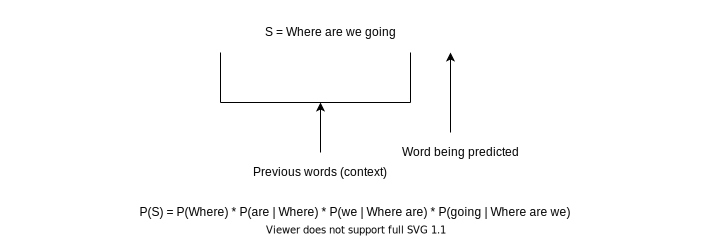
\includegraphics[width=0.8\textwidth]{figures/lm.pdf}
  \caption{Example of a word prediction by using chain rule.}
  \label{chain_rule}
\end{figure}

An example in the Figure \ref{chain_rule} shows how to predict probability of a word given previous words. A subsequence (context) may consist of a very large number of words and the likelihood that such subsequence is found in a corpus is very small. It is a main problem in language models, which is called \textbf{data sparsity}.

Data sparsity is the phenomenon of not observing enough data in a corpus to model language accurately. The solution to resolve this issue is to make the assumption that the probability of a word depends only on the previous \textit{n} words and use \textbf{N-gram model} (N-gram is a sequence of N words).

\begin{table}[t]
  \centering
   \begin{tabular}{|c|c|} 
   \hline
    Hi & 1-gram \\
   \hline
    New York & 2-gram \\
   \hline
   The Three Musketeers & 3-gram \\
   \hline
   She is studying IT & 4-gram \\
   \hline
   \end{tabular}
   \caption{The example of N-grams.}
  \label{tab:n_gram}
\end{table}

The n-gram ``She is studying IT'' from the Table \ref{tab:n_gram} does not occur as often in texts of corpus as n-grams ``Hi'', ``New York'' and ``The Three Musketeers''. Knowing a probability to the occurrence of an N-gram in a sequence of words can be useful, because it can help to decide which N-grams can be chunked together to from single entities (like ``New York'' chuncked together as one word). It can also help make next word predictions. For example, ``tea'' is more likely than ``ball'' in the phrase ``I would like to drink''.

\section{Dialogue systems} 
The ability to communicate with machines in a natural language is a long-standing dream of mankind. Today's dialogue systems often encounter criticism. There are many scientific works on creating more natural dialogue systems. Markus M. Berg defines a natural dialogue system in \cite{berg2014modelling} as ``a form of dialogue system that tries to improve usability and user satisfaction by imitating human behaviour''. It affects the features of human-to-human dialogue (for example, topic changes, sub-dialogues) and seeks to integrate them into dialogue systems for human interaction with the machine. Open-ended natural dialogue systems still have flaws in generating a response to the user.

As noticed in \cite{stent2005evaluating}, the main task of NLG is to select, inflect and order words ``to communicate the input meaning'' as completely, clearly and fluently as possible in context. That's why it is necessary to control not only syntactic correctness of output but also if output is appropriate or felicitous in a given context. A good generator usually relies on several factors:
\begin{itemize}
  \item \textbf{adequacy} (a sentence that is ambiguous or not contains communicates meaning in the input, is \textbf{not} adequate (an example in the Table \ref{tab:adequacy_prob}))  
  \item \textbf{syntactic correctness} (an example in the Table \ref{tab:syntactic_corr_prob})
  \item \textbf{repetition} (self-repetition across utterances and with utterances, repeating the conversational partner (an example in the Table \ref{tab:repetition_prob}))
  \item \textbf{response-relatedness} (efficacy in context (an example in the Table \ref{tab:response_relatedness_prob}))
  \item \textbf{variation} (there are 2 basic forms of variation: \textit{word choice variation} and \textit{word order variation} for enriching speech)
\end{itemize}

\begin{table}[t]
\centering
 \begin{tabular}{|p{0.5cm}|p{8cm}|} 
 \hline
 1 & More phones have games on them than this one. \\
 \hline
 2 & Why a mouse when it spins? \\
 \hline
 \end{tabular}
 \caption{A problem of adequacy shows that a response can be grammatically and syntactically composed correctly, but this sentence does not make sense.}
\label{tab:adequacy_prob}
\end{table}

\begin{table}[t]
\centering
 \begin{tabular}{|p{0.5cm}|p{8cm}|} 
 \hline
 1 & They IS going to school. \\ 
 \hline
 2 & It depends AT you. \\
 \hline
 \end{tabular}
 \caption{A problem of syntactic correctness.}
\label{tab:syntactic_corr_prob}
\end{table}

\begin{table}[t]
\centering
 \begin{tabular}{|c|} 
 \hline
  -Yes, I'm studying law at the moment.\\
  - Good. \\
  - I like playing the piano. \\
  - Good. \\
 \hline
 \end{tabular}
 \caption{A problem of repetition makes conversation boring.}
\label{tab:repetition_prob}
\end{table}

\begin{table}[t]
\centering
 \begin{tabular}{|c|} 
 \hline
 -Do you go get coffee often? \\
 -I am a musician. \\
 \hline
 \end{tabular}
 \caption{A problem of response-relatedness shows that the answer to the question does not make a sense in this context and it spoils the impression of the conversation.}
\label{tab:response_relatedness_prob}
\end{table}

An example in the Table \ref{tab:var_example} shows all types of variation. Sometimes this factor can be syntactically incorrect or unclear, what you can see in the forth sentence. In fifth sentnecne a variation changed the meaning of part of the sentence. In addition, the variation may add or remove meaning possibilities.

\begin{table}[t]
\centering
 \begin{tabular}{|p{0.5cm}|p{8cm}|} 
 \hline
 \# & Example \\
 \hline
 1 & I bought movie tickets on Tuesday. \\ 
 \hline
 2 & I got movie tickets on Tuesday. \\
 \hline
 3 & On Tuesday I bought movie tickets. \\
 \hline
 4 & On movie Tuesday tickets I bought. \\
 \hline
 5 & I bought tickets for the Tuesday movie. \\ 
 \hline
 \end{tabular}
 \caption{The example of sentences' variation.}
\label{tab:var_example}
\end{table}

The main problem in text generation is a language style, which makes a response to an user more human. Language style is defined as the choice of words used by a specific group of people when they speak. Some people use obscene speech, some use a lot of expressive means or jokes to make speech more emotional. This is what distinguishes people and makes their communication more interesting, but at the same time this is the most difficult task for NLG - the ability to generate different communication styles.

\chapter{Approaches to building NLG}
NLG evolution from templates to dynamic generation of sentences took a lot of time and models developed along with it. Corpus-based generation uses a generative probabilistic model what can be implemented in many ways. A lot of simple corpus-based NLG models are based on recurrent neural networks (RNN) and sequence-to-sequence (seq2seq) model, which basically contains a encoder-decoder structure.

\section{Neural Networks}
//TODO

\section{Recurrent neural network (RNN)}

\begin{figure}[hbt]
  \centering
  \includegraphics[width=0.5\textwidth]{figures/rnn.pdf}
  \caption{Architecture of a recurrent neural network, where coefficient \textbf{h} is a hidden layer, \textbf{x} is an input and \textbf{o} is an output. Coefficient \textbf{w} is a weight, what is transformed to produce a sensible output.}
  \label{rnn}
\end{figure}

Recurrent Neural Network are a type of Neural Network where the output from previous step are fed as input to the current step. This allows it to exhibit temporary dynamic behavior. RNNs can use their internal state (memory), which captures information about what has been calculated so far, to process inputs of variable lengths. RNNs are called \textit{recurrent} because they perform the same task for each element of the sequence, and output depends on previous computations.

The architecture of RNN is illustrated in Figure \ref{rnn}, 
Neural networks are computing systems that are inspired by biological neural networks. A "neuron" is a mathematical function that classifies and collects information according to a specific architecture. A neural network contains layers of interconnected "neurons". RNN takes series of input with no predetermined limit on size. Recurrent neural network passes each item of the sequence through a feedforward network and stores the information from the previous step. In each iteration this model calculates the probability of the next item with using information in the memory.



The RNN-based models have been used for NLG as an end-to-end training network \cite{network_nlg} and a training model with semantic aggregation \cite{rnn_nlg}. 

Nowadays RNN networks almost are not used in NLG, because it has problems with vanishing and exploding gradient. The long-term information travels sequentially  through all cells before getting to the present processing cell. This means, that it can be easily corrupted by being multiplied many time by small or big numbers. Other problem of RNN is that they are not hardware friendly, it takes a lot of resources to train and run this network. More information about difficulties of training RNN you can find in \cite{rnn_difficulties}.


\section{Long short-term memory (LSTM)} 

\begin{figure}[hbt]
  \centering
  \includegraphics[width=0.3\textwidth]{figures/lstmCell.pdf}
  \caption{A cell in an LSTM network.}
  \label{lstm}
\end{figure}

LSTM networks are a special kind of RNN, capable of learning long-term dependencies. All recurrent neural networks have the form of a chain of repeating modules of neural network. LSTM network also has this chain structure, but the repeating module has a different structure. 

In Figure \ref{lstm} each line carries an entire vector from the output of one node to the inputs of others. The circles represent pointwise operations, while rectangles are learned neural network layers. Lines merging denote concatenation, while a line forking denote its content being copied and the copies going to different locations.

This model resolved a problem with vanishing gradient, but still the capacity of the LSTM memory is limited, because of inherently complex sequential words' paths from the previous unit to the current unit. The same complexity results in high computational requirements that make LSTM difficult to train or parallelize.

\section{Attention}
//TODO

\section{Transformer} 

\begin{figure}[hbt]
  \centering
  \includegraphics[width=0.5\textwidth]{figures/transformer.png}
  \caption{The architecture of the Transformer \cite{transformer}.}
  \label{transformer}
\end{figure}
Transformer is a relatively new architecture, which proposes a "self-attention mechanism". This model was introduced in the paper "Attention is all you need" \cite{transformer} in 2017. The advantage of this model is a constant number of operations, which simplifies the parallelization of processes. The Transformer uses the representation of all words in context without compressing all information into a single fixed-length representation that allows the system to handle longer sentences without the skyrocketing of computational requirements. 

The architecture of the Transformer is illustrated in Figure \ref{transformer}. The Transformer consists of a stack of encoders (on the left) for processing inputs of any length and another set of decoders (on the right) to output the generated sentences. The inputs and output are first embedded into an n-dimensional space since we cannot use strings directly. The Transformer cannot remember how sequences are fed into a model, because of it positions are added to the embedded representation (n-dimensional vector) of each word.

\chapter{Datasets and Evaluation methods}
A good corpus is very important for successful Natural Language Generation. Dialogue systems require training data in the format of people text conversation, for example, non-fiction or movie reviews are not suitable for this. Large volumes of training data improves the decision-making ability of NLG model, so those models can use it to figure out patterns. Quality is more important for training data than the quantity of data points. Unfortunately, there are not a lot of datasets available for training NLG models, due to the high cost of creating quality datasets. 

In my bachelor thesis I am using 2 different dataset (Twitter data and Persona-Chat). 

\subsection{Persona-Chat}
\begin{table}[t]
\centering
  \begin{tabular}{|p{8cm}|p{4cm}|} 
  \hline
  Average length of  your persona description: & 6.331842242600462 \\
  \hline
  Average length of partner's persona description: & 6.321163335493196 \\
  \hline
  Average length of the first person's utterances: & 11.418615621053272 \\
  \hline
  Average length of the second person's utterances: & 11.929411585690591 \\
  \hline
  Number of your persona description's sentences: & 40239 \\
  \hline
  Number of partner's  persona description's sentences: & 40126 \\
  \hline
  Number of the first person's utterances: & 65719 \\
  \hline
  Number of the second person's utterances:  & 65719 \\
  \hline
  Number of dialogues & 8938 \\
  \hline
  \end{tabular}
  \caption{Persona-Chat statistics}
\label{tab:persona_chat}
\end{table}

\begin{figure}[hbt]
  \centering
  \includegraphics[width=0.9\textwidth]{figures/persona_chat.png}
  \caption{Example dialogue from the Persona-Chat dataset \cite{persona_chat}}
  \label{persona_chat}
\end{figure}

\begin{figure}[hbt]
  \centering
  \includegraphics[width=0.9\textwidth]{figures/persona.png}
  \caption{Example of original and revised personas \cite{persona_chat}}
  \label{revised_persona}
\end{figure}

\begin{figure}[hbt]
  \centering
  \includegraphics[width=0.6\textwidth]{figures/persona_desc.png}
  \caption{Histogram of your persona description lengths}
  \label{histogram_persona_desc}
\end{figure}

\begin{figure}[hbt]
  \centering
  \includegraphics[width=0.6\textwidth]{figures/partner_desc.png}
  \caption{Histogram of partner's persona description lengths}
  \label{histogram_partner_desc}
\end{figure}

\begin{figure}[hbt]
  \centering
  \includegraphics[width=0.6\textwidth]{figures/uttr1_length.png}
  \caption{Histogram of utterances' lengths of the first person}
  \label{histogram_uttr1_length}
\end{figure}

\begin{figure}[hbt]
  \centering
  \includegraphics[width=0.6\textwidth]{figures/uttr2_length.png}
  \caption{Histogram of utterances' lengths of the second person}
  \label{histogram_uttr2_length}
\end{figure}

Persona-Chat models normal conversation when 2 people meet for the first meet and try to get know each other better. The aim of the dialogue is to learn about interests of another person, find common ground and discuss their hobbies. The task involves both asking and answering questions. 

Persona-Chat dataset consists of small conversations between 2 crowdworkers from Amazon Mechanical Turk who were randomly paired and asked to act the part of a given provided persona (randomly assigned, and created by another set of crowdworkers). The data collection consists of persona chat (each dialogue has 6-8 turns), personas (set of 1155 possible personas, each consisting of at least 5 profile sentences), revised personas to avoid word overlap, because crowdworkers sometimes could repeat profile information in a chat(example you can see in the Figure \ref{revised_persona}). In turn-based dialogue each message consists of a maximum of 15 words. All statistics are presented in the Table \ref{tab:persona_chat} Example of Persona-Chat dialogue you can see in Figure \ref{persona_chat}. 


\subsection{Twitter}
Twitter dataset contains message-response pairs from Twitter. Example of these data you can see in the Table \ref{tab:twitter_chat}. 

\begin{table}[t]
\centering
 \begin{tabular}{|p{2cm}|p{8cm}|} 
 \hline
 \multicolumn{2}{|c|}{Example} \\
 \hline
 Person 1 & yeah i'm preparing myself to drop a lot on this man, but definitely need something reliable \\ 
 \hline
 Person 2 & yeah dude i would definitely consider a daniel defence super reliable and they are just bad ass \\
 \hline
 Person 1 & besides if trump say his condolences it won't sound genuine, ex: (dwayne wade cousin) it will sound all political and petty \\
 \hline
 Person 2 & yea you right. but we do live in a world where republicans will harass obama about a birth certificate but won't say \\
 \hline
 \end{tabular}
 \caption{The example of Twitter message-response pairs}
\label{tab:twitter_chat}
\end{table}

\chapter{Other}

Non-task-oriented dialogue system

The aim of task-oriented dialogue systems is to complete specific tasks fo user, non-task-oriented dialogue systems focus on conversing with human on open domains. 

//TODO: Info about datasets

//TODO: Info about evaluation metrics

//TODO: Description of baseline

//TODO: NLP vs Computation linguistic

